\documentclass[final]{article}

% if you need to pass options to natbib, use, e.g.:
% \PassOptionsToPackage{numbers, compress}{natbib}
% before loading nips_2017
%
% to avoid loading the natbib package, add option nonatbib:
% \usepackage[nonatbib]{nips_2017}

\PassOptionsToPackage{compress,authoryear,round}{natbib}
\usepackage{nips_2017}

% to compile a camera-ready version, add the [final] option, e.g.:
% \usepackage[final]{nips_2017}

\usepackage[utf8]{inputenc} % allow utf-8 input
\usepackage[T1]{fontenc}    % use 8-bit T1 fonts
\usepackage{hyperref}       % hyperlinks
\hypersetup{colorlinks=true,linkcolor=black,citecolor=black,filecolor=black,urlcolor=black,
            plainpages=false,pdfpagelabels,breaklinks=true,
  pdftitle    = {Brain Tumour Segmentation with Random Forest and U-Net},
  pdfsubject  = {},
  pdfauthor   = {Shuhan Xiao and Alexander Kugele},
  pdfkeywords = {} ,
  pdfcreator  = {pdflatex},
  pdfproducer = {}
}
\usepackage{url}            % simple URL typesetting
\usepackage{booktabs}       % professional-quality tables
\usepackage{amsfonts}       % blackboard math symbols
\usepackage{nicefrac}       % compact symbols for 1/2, etc.
\usepackage{microtype}      % microtypography
\usepackage{amsmath}
\makeatletter
\providecommand*{\input@path}{}
\g@addto@macro\input@path{{fig/}{../figures/}}
\makeatother

\usepackage{graphicx}
\graphicspath{{fig/}{../figures/}}


\usepackage{enumitem}
\usepackage{cleveref}

\title{Brain Tumour Segmentation with Random Forest and U-Net}

\author{
  Alexander Kugele \\
  Heidelberg University \\
  Matrikel-Nr: 3150330\\
  Physics, M.Sc. \\
  \href{mailto:a.kugele@stud.uni-heidelberg.de}{a.kugele@stud.uni-heidelberg.de}\\
  \And
  Shuhan Xiao \\
  Heidelberg University \\
  Matrikel-Nr.: 3160697 \\
  Physics, M.Sc. \\
  \href{mailto:shuhan.xiao@stud.uni-heidelberg.de}{shuhan.xiao@stud.uni-heidelberg.de}\\
}

\begin{document}

\maketitle

\begin{abstract}
This report compares two methods to segment 2D brain tumour images: A random
forest and a U-Net. It is found that without manual tuning, both methods are
comparable in their segmentation accuracy, achieving Dice scores of $65.9 \%$
and $69.3 \%$ respectively. However, training and inference time of the U-Net
are significantly smaller and training larger datasets is possible more easily.
\end{abstract}

\section{Introduction}
An important task of image processing and image analysis is semantic segmentation, which assigns a class label to each pixel of an image by combining information about the intensity value of the pixel itself as well as its adjacent pixels. One of the most challenging application of image segmentation is the segmentation of biomedical images. It faces the problem that often the appearance of the objects of interest can be highly variable. Especially in medical imaging there might also be variations in image quality, for example caused by motion artefacts and intensity inhomogeneity. \\

This project focusses on the segmentation of gliomas, which are the most common type of tumours, accounting for 81$\%$ of all malignant tumours found in both children and adults \citep{ostrom2014}. Gliomas are categorised into low-grade gliomas (LGG) and high-grade gliomas (HGG) according to their rate of growth and prognosis for the patient.\\
The tumours are usually diagnosed using magnetic resonance imaging (MRI). The advantage of MRI is that it is a non-invasive imaging technique. Additionally, different image contrasts by using different acquisition techniques, i.e. types of scans. Commonly, T$_1$-weighted (T1), T$_1$-weighted contrast enhanced (i.e. using the contrast agent gadolinium) (T1c), T$_2$-weighted (T2) and Fluid-Attenuated Inversion Recovery (FLAIR) images are acquired in multimodal MRI protocols and used for diagnosis, as they provide information about different properties about the tissue.
\\
A challenge of segmenting gliomas is that the tumours are highly heterogeneous, often have no clear defined edge and have variable sizes, shapes and locations. The boundaries of LGG tumours are particularly difficult to detect. This is why the usually trained professionals are required to manually label the images. The labelling is however time consuming and not reproducible.\\
Another reason why tumour segmentation is essential is its many applications:\\
\begin{itemize}
\item diagnosis
\item categorisation of tumour and state of disease
\item prognosis (e.g. to predict survival)
\item localisation of tumour for treatment (radiotherapy, surgery)
\item monitoring the development and growth
\end{itemize}
Tumour segmentation is required to have a high accuracy. It is also important that it is quantitative, automatable and reasonably fast. \\
Numerous of techniques have been developed for the task of segmentation so far. The goal of this student project is to adapt two of those techniques to our problem of tumour segmentation and to the hardware available to us: the random forest and the U-Net.\\
The random forest \citep{ho1995} is an ensemble methods, combining several decision trees. It developed to deal with mulitclass problems and was shown to be robust outliers and less likely to overfit.\\
The U-Net was originally applied the to cell tracking \citep{ronneberger2015u}. It is a type of fully convolutional network and specifically developed for segmenting biomedical image. \\
These techniques are further described in \cref{sec:methods}. We have applied our methods to the Multimodal Brain Tumor Image Segmentation Benchmark (BRATS 2015), which is further described in \cref{sec:dataset}. Our results and comparison of the two techniques are presented in \cref{sec:results}.
\section{Related Work}  \label{sec:related}
Both random forest and U-Nets have been previously applied to segment tumours in the BRATS challenge. \\

\cite{pinto2015} applied their extremely randomized forest to the BRATS 2013 dataset using both appearance- and context-based features and achieved a Dice score of 83$\%$ and a sensitivity score of 83$\%$ for the whole tumour region. \\ Random forests were also used by \cite{maier2015}, who obtained a Dice and sensitivity score of 84$\%$ and 85$\%$ respectively for the whole tumour and only LGG cases. Their features include the intensity, gaussian, local histogram, hemispheric difference and center distance.\\
A U-net combined with data augmentation has been previously used in the BRATS 2015 challenge by \cite{dong2017} successfully. They achieved a Dice score of 81$\%$ for the complete LGG tumours. \\
With an an ensemble of a DeepMedic architecture consisting of fully 3D multi-scale convolutional neural networks (CNN), three fully convolutional networks (FCN), and two 3D U-Nets, \cite{brats2017short} obtained the best overall result of the most resent BRATS challenge in 2017 \citep{bakas2017advancing} with their so called Ensembles of Multiple Models and Architectures. Their method lead to a Dice score of 90.1$\%$ and a sensitivity score of 89.5$\%$ for the whole tumour.

\section{The Dataset} \label{sec:dataset}

\subsection{General Information}
Image segmentation is primarily done in two ways: Either designing an algorithm
from first principles or using available data to train an algorithm. As for
this challenge, designing an algorithm without data is very difficult, the
method of choice is training an algorithm from data. For the Multimodal Brain
Tumor Image Segmentation Benchmark \citep{BRATS} in 2015, 3D MR tumour scans
where collected from the BRATS 2012 and BRATS 2013 challenge and from the NIH
Cancer Imaging Archive (TCIA).\\ In total, data for 55 low-grade glioma patients
and 220 high-grade glioma patients is provided. The data is a 16-bit 3D scan of
shape (depth=155, height=240, width=240), where all datasets have been aligned
to the same anatomical template and interpolated to 1 mm$^3$ voxel
resolution. For each patient, four scan types are available: T1, T1c, T2 and
FLAIR. In the case of the BRATS data, the labels are from expert annotations of
one to four raters. The TCIA data labels were obtained by fusing the results of
multiple segmentation algorithms from the BRATS 2012 and BRATS 2013 challenge
and reviewed by expert raters.\\
Four classes are predefined:
\begin{enumerate}[label=\arabic*),topsep=0pt]
  \setcounter{enumi}{-1}
\item background
\item necrosis
\item edema
\item non-enhancing tumour
\item enhancing tumour
\end{enumerate}
Each 3D image for each scan type is saved in a separate \verb+.mha+ file. The
average size per file is about 2.2 MB, leading to approximately
 2.2 MB $\cdot 275 \cdot 4 =$ 2420 MB of compressed data.
Uncompressed, the data size increases to over 100 GB. In
\cref{fig:dataex}, examples for LGG and HGG and the different scan types are
shown.

\begin{figure}[h]
\centering
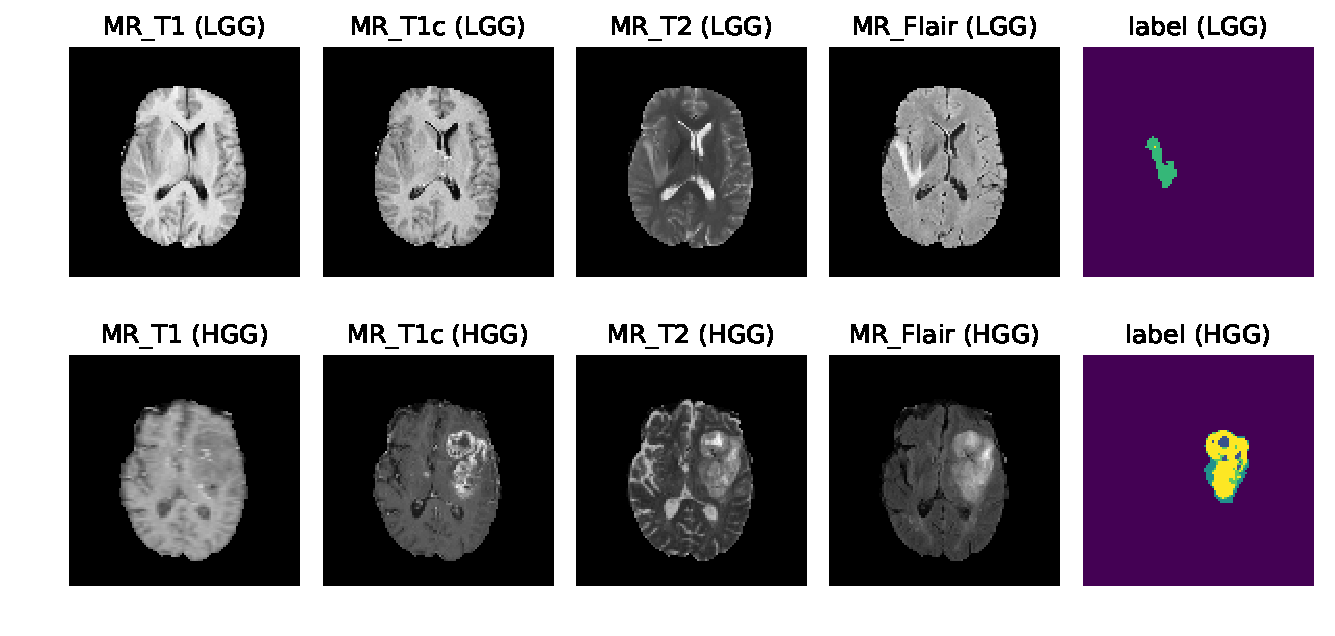
\includegraphics[width=0.99\linewidth]{scan_types_both}
\caption{Dataset examples. \textit{Top:} Low-grade glioma tumour. The structure
is primarily visible in the Flair scan. \textit{Bottom:} High-grade glioma
tumour. The structure is richer and the different scan types help in
differentiating the different types of tumour.}
\label{fig:dataex}
\end{figure}

\subsection{Utilizing the Dataset}
The given images are sliced 3D scans. As we want to do segmentation in two
dimensions, we just take each slice as a separate input image. In total, this
are $155\cdot275\cdot4 = 170500$ input images. This full dataset proved too be
to large to use it for training. After trying out multiple subsets, it was
decided to use only the LGG part of the dataset and to sort out images where
the tumour to background ratio is less than $0.1\%$. We only used FLAIR images, which provide the most meaningful information about the tumour structure as illustrated in \cref{fig:dataex}. Registration, which would have been inaccurate due to the varying resolutions of the scans, was therefore not necessary.\\ 

This dataset only takes
110 MB compressed on disk. We split this dataset of 3315 images further
up into a training set of 2652 images ($80\%$) and a test set of 663 images.
This dataset is used for both the random forest and the U-Net. The classes are
reduced from five to two: background and tumour. Loading 10 images in the memory
of the GPU for training takes about 3 GB. For the random forest, using
1000 images at once takes about 30 GB of RAM.

\section{Methods} \label{sec:methods}
\subsection{Random Forest}
The random forest is a set of decision trees, where each tree is fitted to a
random subset of the data and predictions are made by taking averages over the
predictions of individual trees. More precisely, given $N$ data points, $N$
points are sampled at random with replacement from the data. These are then
used to train a decision tree. This kind of sampling is called bagging. The
samples that are not used for the training of a decision trees are so-called
out-of-bag samples. These can be used to test the generalization accuracy of
the training.\\

Training of each decision tree in scikit-learn is done with the Classification
and Regression Tree (CART) algorithm.  Before explaining the training
algorithm, the Gini impurity is explained. This measure is used to determine
the next split in a tree. Generally, it can be calculated as
\begin{equation}
G_i = 1 - \sum_{k=1}^{n}p_{i,k}^2
\end{equation}
where $i$ is the node index, $k$ is the class label and $p_{i,k}$ is the ratio
of class $k$ to all classes in the node. The CART algorithm uses a loss based
on this measure
\begin{equation}
J(k, t_k) = \frac{m_L}{m}G_L + \frac{m_R}{m}G_R
\end{equation}
such that it finds for each current leaf a class and a threshold such that the
impurity is minimized for the left and the right leaf to be added. This is done
until the impurity cannot be further reduced or the maximum depth is reached.
The default parameter in scikit-learn is \verb+max_depth=None+, meaning it goes
as deep as it can. This can lead to large trees. An example of one tree after
training is shown in \cref{sec:treevis}, where each small orange or blue dot is
a single node.

\subsubsection{Features} \label{sec:features}
A random forest classifies each pixel separately. Therefore, using only the
pixel intensities would only give a good classification if the tumour can be
identified on a single-pixel level. To include information about the local
structure, multiple features are defined, such that each input pixel is an
N-dimensional vector.\\ The features we chose for this task are:
\begin{enumerate}
\item Gaussian filter
\begin{itemize}
\item Convolution with a Gaussian kernel
\item Smoothes the image
\end{itemize}
\item Laplacian of Gaussian (LoG) filter
\begin{itemize}
\item Convolution with the Laplacian of a Gaussian kernel
\item highlights edges (edges are 0)
\end{itemize}
\item Gaussian gradient magnitude filter
\begin{itemize}
\item Convolution with the gradient of a Gaussian kernel
\item highlights edges (edges are extrema)
\end{itemize}
\item Eigenvalues of the Hessian matrix
\begin{itemize}
\item determines the surface concavity
\end{itemize}
\item Eigenvalues of the structure tensor
\begin{itemize}
\item Summarizes gradient direction
\end{itemize}
\item Equalized histogram
\begin{itemize}
\item Enhances contrast
\end{itemize}
\end{enumerate}

Except for the equalized histogram, they all share the tuneable kernel width
$\sigma$, which is set to $\{0.3, 0.7, 1., 3.5\}$. In total, $N=29$ filters are
used. In \cref{fig:features}, the features are shown for one example image of
the dataset for $\sigma = 0.3$. The tumour region in the bottom left can be
clearly identified for the Gaussian (bright), Laplacian of Gaussian (dark) and
the equalized histogram (bright). However, for other examples the tumour is also
pronounced in the other features.

In principle one could also utilize the different scan types as features.
However, the dataset is already very big and therefore it was decided to not
take the other scan types as features. This also allows for a fair comparison
between the random forest and the U-Net, as they are then trained with the same
dataset.\\

\begin{figure}
\centering
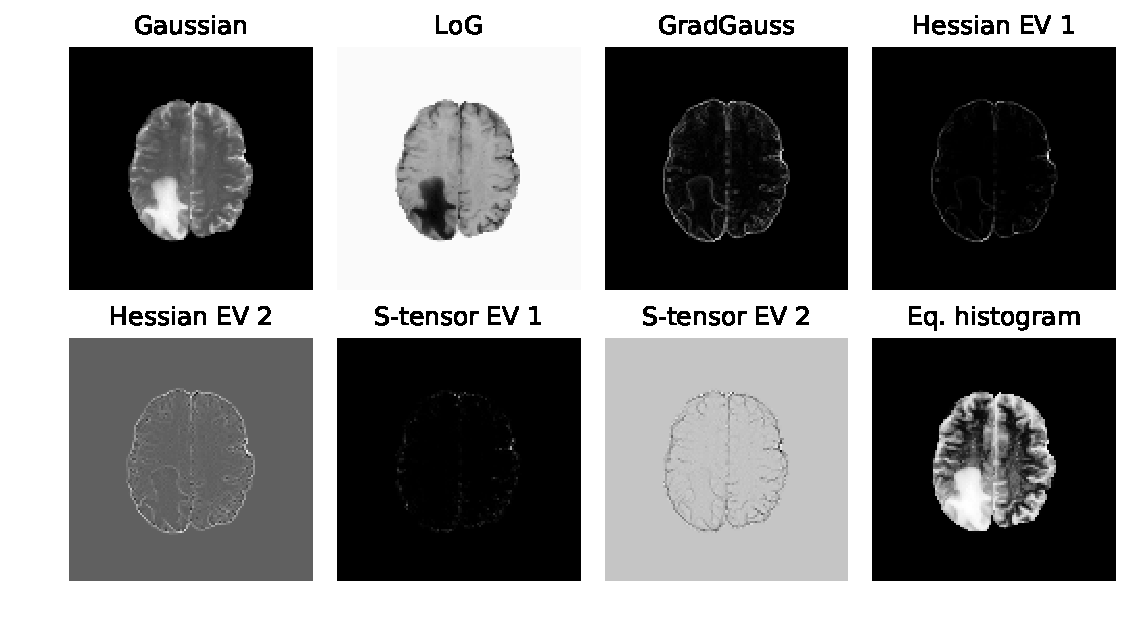
\includegraphics[width=0.99\textwidth]{features}
\caption{Features for the random forest. The Gaussian, Laplacian of Gaussian
and the equalized histogram enhance the tumour region. In this example, the
eigenvalues of the structure tensor and the Hessian matrix are not significant
for the classification. However, they improved the classification on a small
test set and therefore are also kept.}
\label{fig:features}
\end{figure}
\subsection{U-Net}
\begin{figure}[h]
\centering
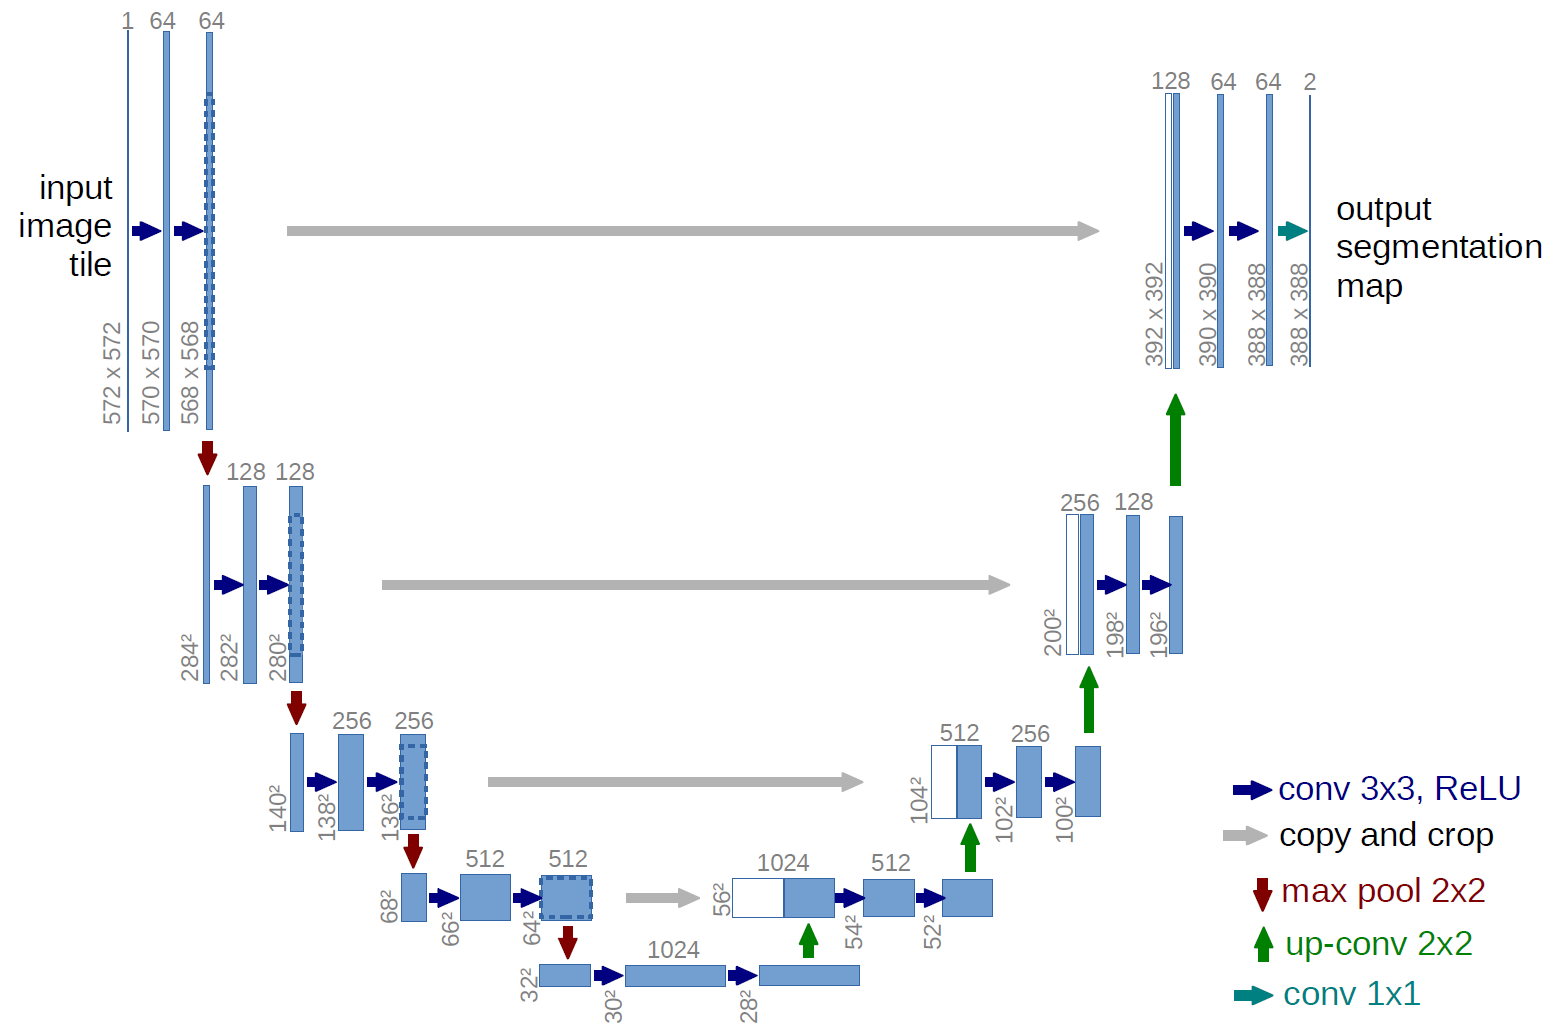
\includegraphics[width=0.99\textwidth]{u_net}
\caption{U-shaped architecture of the original U-net. \citep{ronneberger2015u}}
\label{fig:u-net}
\end{figure}
We implemented a U-Net for our problem, which is based on a fully convolutional network by \cite{Long14}. \cite{ronneberger2015u} showed that the U-net requires only a few training images when combined with data augmentation. We based our implementation on the versions of \cite{zijundeng} and \cite{jaxony}, with a few additional modifications.\\

The distinct u-shaped architecture of the original U-Net with its skip-connections is shown in \cref{fig:u-net}. It has two symmetric paths: a contracting (down-sampling) and an expanding (up-sampling) path, each originally with five blocks. \\
We used a U-Net with the depth of only four blocks for each path instead to increase training speed and as the size of our input images was only $240 \times 240$. Our lowest resolution of the feature maps with $30 \times 30$ pixels is still smaller than the resolution of the original U-Net with $32 \times 32$ pixels. 
In total, our whole U-Net has only 18 convolutional layers instead of 23.\\

The contracting path allows to capture context of each pixel and to extract information from different feature levels. In each block two $3 \times 3$ convolutions with stride 1 are performed, each followed by rectified linear unit activation function (ReLU). In contrast to the original U-Net, the images are zero-padded in order to avoid cropping. We also added batch normalisation after each ReLU to improve the gradient flow, allowing higher learning rates and thus increase training speed. Max pooling with stride $2 \times 2$ is then applied for downsampling. This also doubles the number of feature channels up to 512 in after the fourth block, while reducing the spacial information. We used dropout in the forth block to decrease overfitting, as no data augmentation was used.\\
The expanding path is symmetric to the contracting path. In this path, the resolution is increased so that context information is propagated to higher layers. In each block, a concatenation with the corresponding feature map from the contracting path is performed, followed by upsampling with a $2 \times 2$ up-convolution, two zero-padded $3\times 3$ convolutions with stride 1, ReLU activation and batch normalisation. Due to previous padding in the contracting path, no cropping is required here.  The up-convolution halves the number of feature channels while increasing the size of the feature maps. The skip-connections between the two paths allows the combination of spatial information from the contracting path and information about the context from the expanding path. 
\\
In the final layer each feature map with 64 channels is mapped to the number of classes, which is 1 for the case of binary segmentation, by a $1 \times 1$ convolution. \\
After applying an argmax function, or in our binary case a sign function, the output of the network is a pixel-wise (binary) segmention of the input image.

\section{Experiment}

\subsection{Training}
\subsubsection{Random Forest: Batch-mode training}
Using the features defined in \cref{sec:features}, the complete training data
still takes about 70 GB of memory. Therefore, it is decided to train the
random forest sequentially on large chunks of the dataset as suggested in
\cite{batchrf}. The dataset is divided in three batches of about 26 GB
each, assuming that in each large batch, the distribution of features is
approximately equal. Then, we train a random forest on 100 estimators for each
batch. The resulting random forest therefore has 300 estimators. It takes
approximately 15 GB on disk, saved in the pickle format. In scikit-learn,
the \verb+warm_start=True+ parameter of the Random Forest can be used to do
this kind of batch-mode training. \\

Training the random forest took about 13 hours. Storing it on disk takes
about 15 GB in pickled format. Both training time and classifier disk
size can be reduced by setting adjusting the hyperparameters \verb+max_depth+,
\verb+min_impurity_leaf+, \verb+max_leaf_nodes+, \verb+min_samples_split+,
\verb+min_samples_leaf+. However, finding a good setup is also time-consuming
and we mainly want to compare the segmentation accuracy. Therefore, the
standard values are kept. Therefore, loading the classifier takes about
310 s and a single prediction takes about 2-20 s. 
\subsubsection{Training of the U-Net}
The U-Net was trained for 30 epochs with a batch size of 10 images per batch. The weights were intitialised by Xavier initialisation. Instead of the cross-entropy loss used by \cite{ronneberger2015u} we used a loss based on the Dice score (\cref{sec:metrics}), which was also our evaluation metric. We used the Adam Optimizer in pytorch for faster training. Training took 1.5 hours in total with an inference time of 0.5 s per image and a loading time of 20 s. It took a disk space of 0.3 GB and a
memory space of 0.7 GB during inference. 
\begin{figure}[h]
\centering
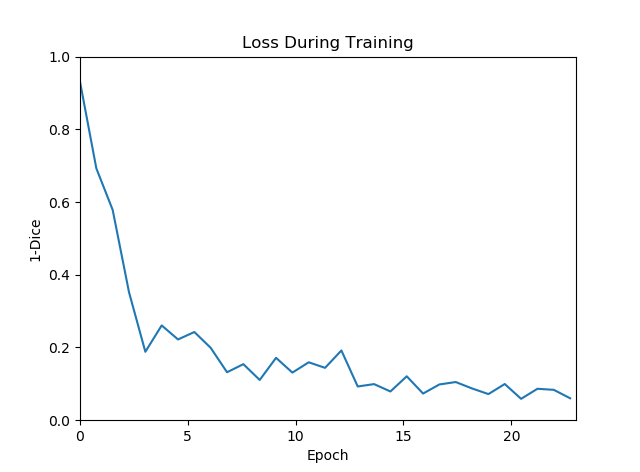
\includegraphics[width=0.79\textwidth]{trainingloss}
\caption{Loss of the U-Net during training. After 30 epochs a loss of approximately 0.1, corresponding to a Dice score of 0.9 for the training set, was achieved.}
\label{fig:rfresults}
\end{figure}
\subsection{Evaluation Metrics} \label{sec:metrics}
For a quantitative comparison we calculated three metric as described by \cite{BRATS}. \\
We used the Dice score $\in [0,1]$ for our evaluation given by
\begin{align}
\mathit{Dice} &= \frac{2|P_1 \cap T_1|}{|P_1|+|T_1|} \\
& = 	\frac{2 \mathit{TP}}{\mathit{FP} + 2 \mathit{TP} + \mathit{FN}},
\end{align}
where $P_1$ and $T_1$ represent the pixels corresponding to the tumour of the prediction and ground truth respectively. \textit{TP}, \textit{FP} and \textit{FN} denote the true positive, false positive and false negative pixels respectively. The Dice score is a measure for the overlap between the tumour regions of prediction and ground truth.
The loss of the U-Net was set to
\begin{equation}
\mathit{Loss} = 1 - \mathit{Dice}.
\end{equation}
We also calculated the sensitivity score (true positive (\textit{TP}) rate or recall) and the specificity score (true negative (\textit{TN}) rate)
\begin{equation}
\mathit{Sensitivity} = 	\frac{\mathit{TP}}{\mathit{TP} + \mathit{FN}}
\end{equation}
and
\begin{equation}
\mathit{Specificity} = 	\frac{\mathit{TN}}{\mathit{TN} + \mathit{FP}}.
\end{equation}
We used these scores because they are able to deal with the class imbalance. In the case of tumour segmentation much more pixels belong to the background (i.e. healthy tissue), so it is more likely that tumour pixels are overlooked.

\section{Results, Comparison and Discussion} \label{sec:results}

In
\cref{fig:rfresults} and \ref{fig:uresults}, an example for the segmentation of test image 84 is shown
together with the box plots for the Dice score, sensitivity and specificity. We obtain similar scores for both techniques.
The mean scores of the random forest are Dice$=65.9 \% $, sensitivity$=77.1 \%$ and
specificity$=99.1 \%$, the mean scores of the U-Net are slightly higher with Dice $=69.3 \% $ and
specificity $=99.4 \%$, the sensitivity$=73.1 \%$ is slightly lower.\\
The scores are also listed again in \cref{tab:scores}, together with the scores of the other methods mentioned in \cref{sec:related}. Compared to the methods \cite{maier2015}, \cite{dong2017} and \cite{brats2017short}, our average performance is significantly worse. It needs to be noted however that the techniques were used for  multi-class segmentation instead of binary segmentation, as we did in our case.

\begin{figure}[h]
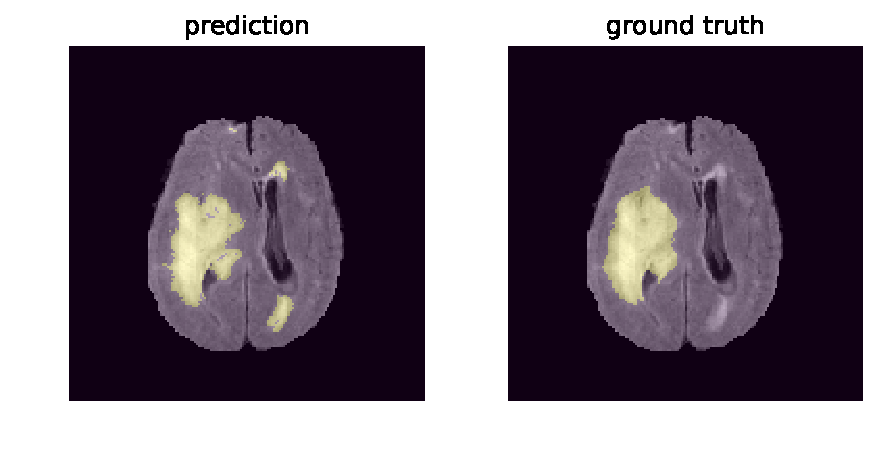
\includegraphics[width=0.49\textwidth]{rf_prediction_84}
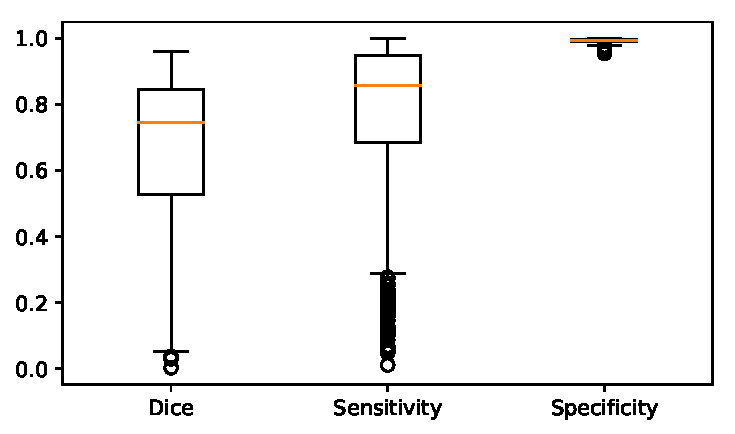
\includegraphics[width=0.49\textwidth]{boxplot_rf}
\caption{Results of the predictions using our random forest. \textit{Left:} Example for a prediction on image 84 of the test set.
The true tumour is segmented very precisely, but other smaller bright areas are
also incorrectly classified as being a tumour. \textit{Right:} Boxplots for the
Dice score, sensitivity and specificity. As most of the images are background,
the specificity is very high and has a low standard deviation. The quantiles
$Q_1$ (25th percentile) to $Q_3$ (75th percentile) span almost over the whole
range of the Dice score and sensitivity. This means that for a single image,
the classification can vary significantly.}
\label{fig:rfresults}
\end{figure}

\begin{figure}[h]
\centering
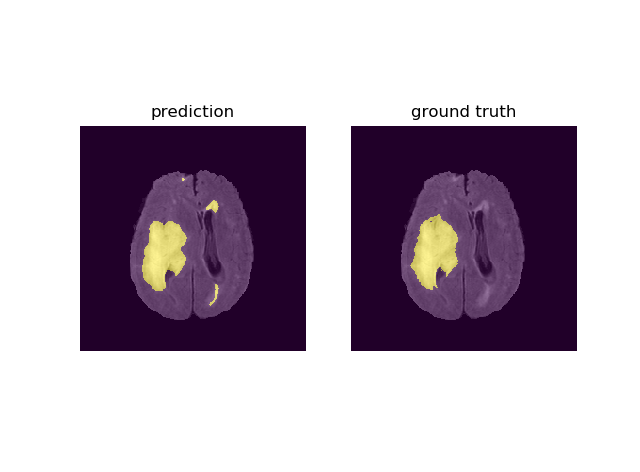
\includegraphics[width=0.49\textwidth]{test_Flair_84}
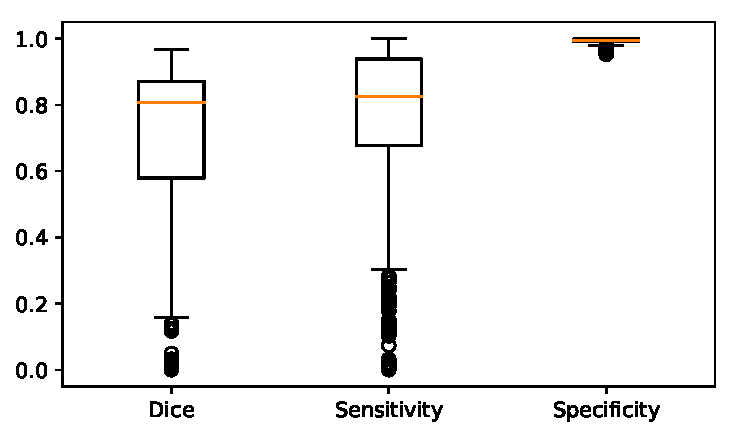
\includegraphics[width=0.49\textwidth]{boxplots}
\caption{Results of the prediction using our U-Net. \textit{Left:} Example for a prediction on image 84 of the test set.
The segmentation of the true tumour is as accurate as for the random forest. The edges of the segmented tumour is smoother that compared to in \cref{fig:rfresults}. The pixels incorrectly classified as tumour pixels, i.e. false positives, are also present in areas with high intensity, but smaller than for the random forest. \textit{Right:} Boxplots for the
Dice score, sensitivity and specificity. Just as for the random forest, the specificity is very high and has a low standard deviation. The median Dice score is slightly higher at about 0.8, the sensitivity score is however slightly lower as in \cref{fig:rfresults}. The outliers all lie below the median, which is why the mean of the Dice and sensitivity scores is in fact lower.}
\label{fig:uresults}
\end{figure}

\begin{table}[h]
\centering
\begin{tabular}{lrrr}

	\toprule
	 & Dice [$\%$] & Sensitivity [$\%$] & Specificity [$\%$] \\
	\midrule
	Random Forest & $65.9$ & $77.1$ & $99.1$ \\
	U-Net & $69.3$ & $73.1$ & $99.4$ \\
	\citeauthor{maier2015} (BRATS 2015, LGG)& $84$ & $85$ & - \\
	\citeauthor{dong2017} (BRATS 2015, LGG) & $84$ & - & - \\
	\citeauthor{brats2017short} (BRATS 2017, winner) & $90.1$ & $89.5$ & - \\
	\bottomrule \\
	
\end{tabular}
\caption{Comparision of Dice score, sensitivity and specificity of the segmentation of the whole tumour between our random forest and our U-Net. The scores of methods by \cite{maier2015}, \cite{dong2017} and \cite{brats2017short} are given as a reference.}  \label{tab:scores}
\end{table}


The cases of our test set where the U-Net performed the worst and best with regard to the Dice score is shown in \cref{fig:goodbad}. The figure also illustrates the strength and weaknesses of the U-Net. In both cases most of the tumour area is labelled as non-enhancing tumour in the ground truth. In the case with the lowest Dice score (top row) the U-Net is not able to detect the upper half of the tumour, but marks it as background (i.e. false negative). The intensity of the tumour appears similar to the normal tissue in the FLAIR image, only the edge has a higher intensity. In the case with the highest Dice score (top row), the intensity of the FLAIR image is visibly higher in the tumour region. The tumour area is detected correctly by the U-Net.\\
This shows that the U-Net is highly sensitive to areas with high intensity, but is not able to detect tumours when the intensity difference is small.

\begin{figure}[h]
\centering
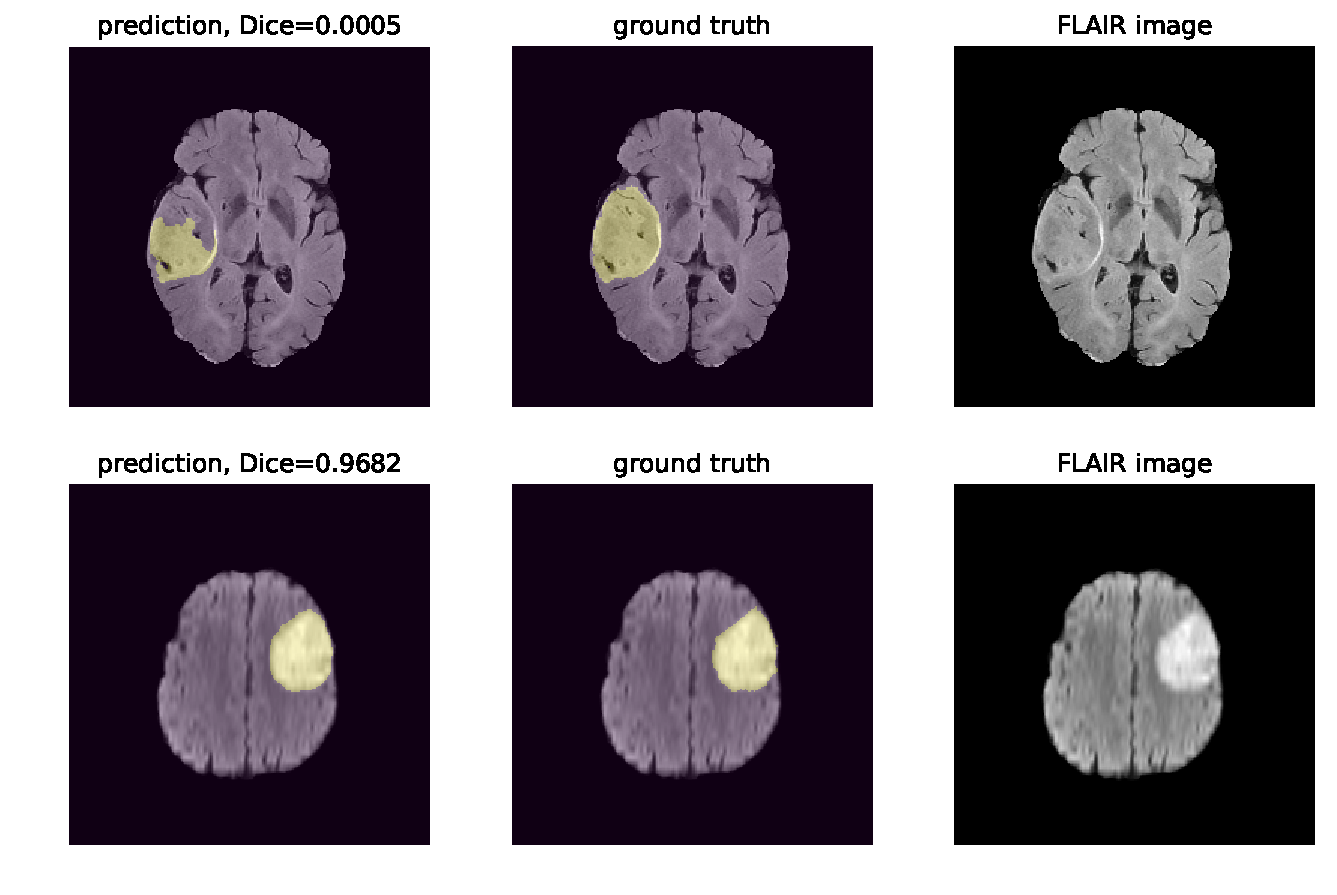
\includegraphics[width=0.99\textwidth]{goodbad_ex}
\caption{Predictions with our U-Net. \textit{Top:} Prediction with overall lowest Dice score. \textit{Bottom:} Prediction with overall highest Dice score.}
\label{fig:goodbad}
\end{figure}
\newpage
\section{Future Work}
Our implementations only dealt with binary segmentation and were only possible to discriminate between tumour/ non-tumour regions. However, there is a larger variation in appearance from class to class, which could be addressed by training our methods on the classes separately.\\ In order to put more emphasis on "harder" examples, which are mainly tumours with a lower intensity contrast, the each training image could be weighted accordingly. \\
The shorter training time of the U-Net leaves room to increase the training data set by for example also include HGG cases or data augmentation. \\
Finally, another possibility is to combine both methods as ensemble and use features from the U-Net for the random forest, similar to the work by \citeauthor{brats2017short}.
\section{Conclusion}
In this project, we tested two approaches to perform tumour segmentation on MRI images, a random forest and a U-Net. \\ 
Even though our techniques were less accurate than other state-of-the-art techniques, we were able to implement, train and test them in a reasonable amount of time, when considering our limited resources. \\
Both techniques lead to similar segmentation accuracies. Training and inference
time with the U-Net are significantly smaller and it is expected to be able to
increase the segmentation accuracy by a deeper U-Net, longer training time,
more training data and hyperparameter tuning. To increase the prediction
accuracy of the random forest, new features have to be introduced. As it is
difficult to decide which features will lead to better results, improving the
U-Net is easier. Also, adding more training data does only lead to a longer
training time for the U-Net, but for the random forest it additionally requires
more memory resources, making this method less flexible.
\newpage
\section{Appendix}

\subsection{Hardware Specifications}
This section lists the hardware details of the machine used to train the random
forest and the U-Net. This makes the given times more comparable to other
systems.
\begin{itemize}
\item Intel Core i5-3550 CPU \@ 3.30GHz
\item Nvidia Geforce GTX 1060 6GB
\item 8 GB RAM
\item 40 GB swap on SSD
\end{itemize}

\clearpage
\subsection{Visualization of a single tree}
\label{sec:treevis}
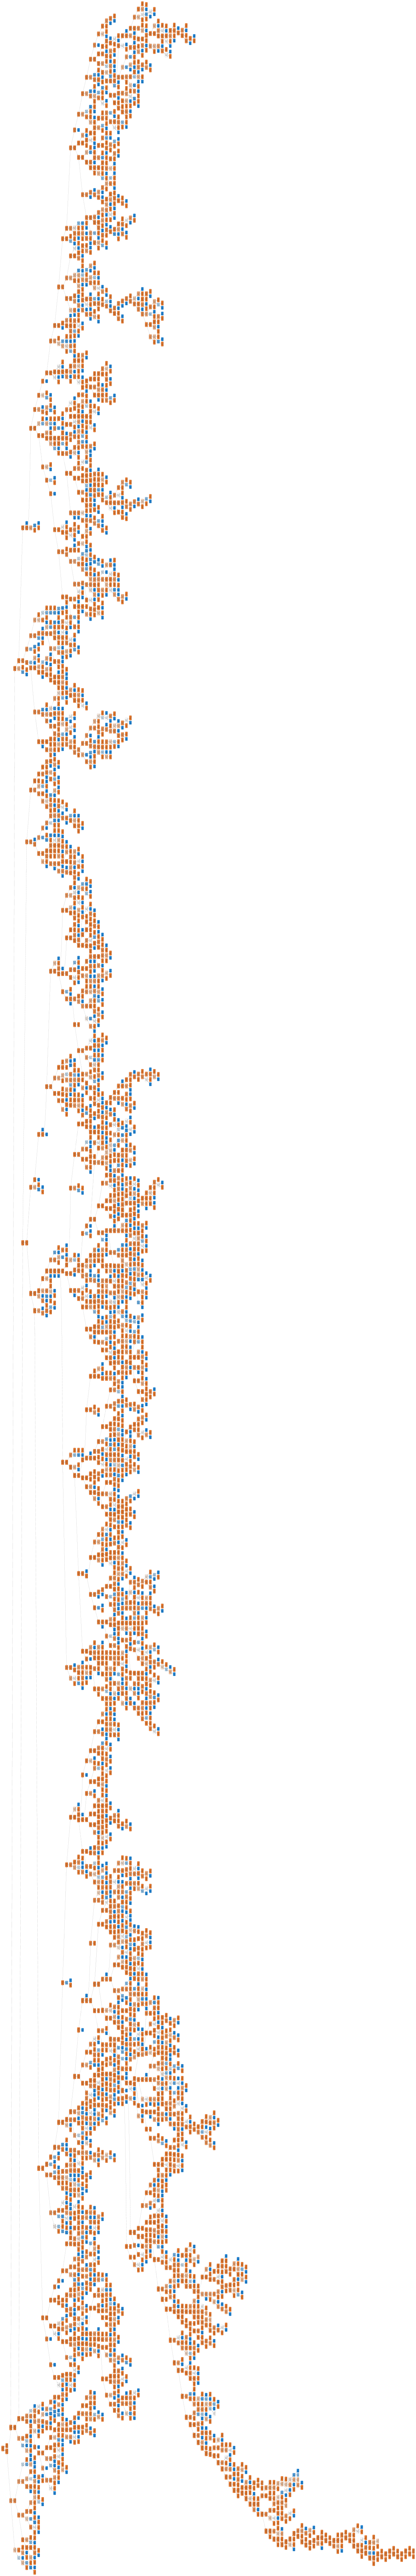
\includegraphics[width=0.94\textwidth,height=0.94\textheight]{Tree4.png}

\bibliographystyle{plainnat}
\bibliography{../biblio}\vspace{0.75in}

\end{document}
